%!TEX root = main.tex

\chapter{Insights on Grover Search Algorithm and its implementation}
\label{chp:grover}

\section{Introduction}

\subsection{Premise}

Our Quantum Max Flow Analysis algorithm described in \cref{chp:mfa}, bases its reason to exist in the fact that a small routine of the algorithm (the search for the next arc to be considered among those coming out of a given node) is done by a quantum computer. It is in fact nothing more than a search in a list (or more generally in a database) of one or more elements that satisfy a certain condition (the arcs that have not been visited yet, i.e. having infinite weight value).

\subsection{The problem}

Let's start noticing that although we have presented in \cref{sec:QSgrover} an implementation of Grover Search in Q\#, it actually works on what is known as ``virtual database''. Alike real databases, virtual (or implicit) ones are not really databases: given $n$ as the number of bits, they are nothing more than the set of integer numbers $\left[0, 2^{n-1}\right]$.

Such a ``database'' can be easily implemented with a quantum register initialized with $H^{\oplus n}$. In this way, whenever the register is measured, it collapses to one of all the possible combinations of its bits (i.e. $\left[0, 2^{n-1}\right]$), being all these combinations all equally probable.

\bigskip

Actually the implementation described in \cref{sec:QSgrover} complies with most of the available literature \cite{Grover:1996:FQM:237814.237866, lavor2003grover}. It is evident that currently most of the works someway related to Grover Search Algorithm are devoted to quantum search on virtual databases. \cite{Broda2016}

\bigskip

Apparently some people agree that Grover is limited to implicit databases, therefore not convenient or even not useful at all for real databases \cite{1425397, Zalka2000, stackexchange1, stackexchange2, stackexchange3}. On the other hand, someone had a deeper study on the algorithm, understanding the mechanism and implementing (at least mathematically) the encoding and the search on a real database. \cite{alsing2011grover}

%\bigskip
%
%We will build on this last paper to answer the questions:
%\begin{itemize}
%	\item Is it correct to use Grover Search for a real database search?
%	\item Is it feasible? (i.e. could an algorithm be devised to do so?)
%\end{itemize}

%TODO an outline of this chapter

\section{The phone book implementation}

The work \cite{alsing2011grover} actually finds a way to encode some elements into a real database. It is done setting a register to an entangled state, as sum of the states corresponding to the elements that we want to encode into the database. This database-register is created by applying a particular matrix to it, in which the database elements are encoded within the rows order. An example is shown in \cref{fig:row_swap}.

\begin{figure}
	\centering
	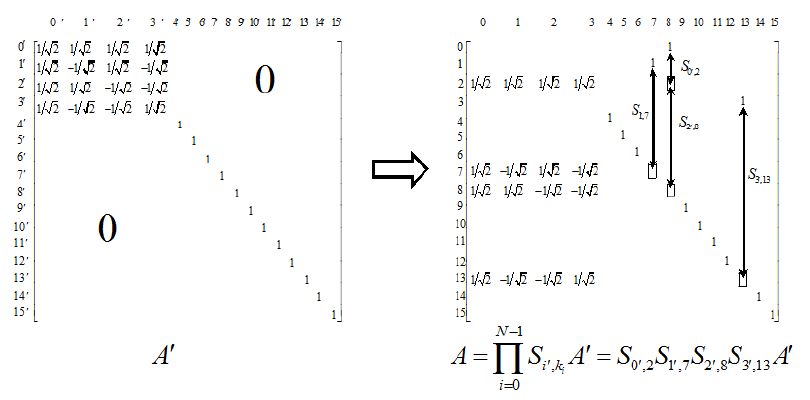
\includegraphics[width=\linewidth]{row_swap}
	\caption{Successive row swapping operations to transform $A'$ in the prime frame to $A$ in the unprimed frame for the specific telephone database example. (credits to \cite{alsing2011grover})}
	\label{fig:row_swap}
\end{figure}

%To obtain this matrix, an identity operator I is enough, a pair of gates H and a matrix that if you multiply it with something simply exchanges the order of the lines of that something.
%
%This last matrix cannot be obtained as a product of simple operators (H, I, X, Y, Z), but must be implemented as logic gates on the individual bits in a more or less complex way. The objective for now is to understand if it is possible to find the combination of logic gates appropriate to reproduce a generic row exchange matrix or, if the thing cannot be automated, a specific instance.
%todo verify

%todo



%\section{Feasibility analysis}

%TODO